\chapter{Обзор работ в области верификации моделей программных систем на языке Си}
Цель данного обзора --- рассмотреть существующие подходы в области верификации моделей крупных программных систем на языке программирования Си, их ограничения и  пределы применимости.

\section{Верификация моделей Си-программ}

Cложность и размер программных продуктов постоянно растут, что приводит к кооперации и повторному использованию существующих программных систем с открытым исходным кодом.
Например, разработчики таких браузеров, как Microsoft Edge, Opera, Amazon Silk, начали использовать проект Сhromium~\cite{chromium}, отказавшись от собственных разработок.
Показательным является применение ядра операционной системы Linux~\cite{linux} при построении информационных систем для портативной электроники, серверов и суперкомпьютеров, программного обеспечения для обслуживания бирж.
Тенденция роста и увеличения сложности в полной мере относится и к программам на языке программирования Си, размер которых исчисляется сотнями тысяч строк кода.
Например, по данным проекта OpenHub на языке программирования Си реализованы компоненты более 50 тысяч проектов свободного программного обеспечения размером в общей сложности более 8 миллиардов строк кода~\cite{openhub}.

Применение крупных программных систем на языке программирования Си при построении информационных систем, к которым предъявляются высокие требования надежности и безопасности, приводит к необходимости применения методов формальной верификации согласно международным стандартам.
В общем виде задача формальной верификации неразрешима согласно теоремам Алана Тьюринга~\cite{turing} и Генри Гордона Райса~\cite{rice}. 
Но на сегодняшний день подходы к решению частных случаев данной задачи активно развиваются.

Методы формальной верификации программ можно разделить на два класса.
Первый класс методов нацелен на доказательство корректности программы относительно набора функциональных требований, формализованных в виде программных контрактов.
Представителем данного классам методов является дедуктивная верификация программ~\cite{Floyd1993, Hoare:1969:ABC}.
Существует много примеров программ, формально верифицированных при помощи данного метода~\cite{Leroy:2009:FVR, seL4, CoCon, CakeML, Davis2015, HOL, FSCQ, CertiKOS}.
Но размер каждой из верифицированных программных систем составляет немногим более десяти тысяч строк кода на языке программирования Си, а в ряде случаев их размер и гораздо меньше.
Трудоемкость процесса верификации велика, например, на верификацию микроядра seL4 размером менее десяти тысяч строк кода на языке программирования Си было затрачено в 5 раз больше усилий, чем на его разработку.
Другой класс методов рассматривает верификацию крупных программных систем на соответствие одному или нескольким требованиям.
Ключевым подходом в данном классе является метод верификации моделей (англ. Model Checking), предложенный Эдмундом Мельсоном Кларком и Эрнестом Алленом Эмерсоном в 1981 году~\cite{MC}.
Ученые были удостоены премии Тьюринга вместе с Иосифом Сифакисом в 2007 году в связи с особой значимостью своего открытия.
История и предпосылки возникновения метода изложены в работе одним из авторов~\cite{Clarke:2008:BMC}.

Направление верификации моделей сегодня включает множество методов и алгоритмов.
В данной работе рассматривается верификация программ, представленных в виде исходного кода на языке программирования Си.
Процесс выполняется полностью автоматически и заключается в построении модели программы и ее проверке при помощи какого-либо алгоритма верификации моделей~\cite{DSilva:2008:SAT}.
Такой подход реализован в инструментах верификации моделей программ (англ. software model checker, software verifier).
Современные инструменты верификации способны проверять требования к программам размером несколько десятков тысяч строк кода на языке программирования Си.

%Прежде чем представить метод проверки требований к крупным программным системам на языке программирования Си требуется рассмотреть ограничения инструментов верификации моделей программ и существующие методы автоматизированного применения данных инструментов.

\section{Инструменты верификации моделей Си-программ}

Первые применяемые на практике инструменты верификации моделей программ появились в начале 2000-х.
Тогда появились такие инструменты, как Blast~\cite{Henzinger:2003:SVB} и Slam~\cite{Ball2004}.
Сегодня сообщество разработчиков инструментов верификации моделей программ выросло и организовалось вокруг ряда таких конференций, как TACAS~\cite{tacas}, ETAPS~\cite{etaps}, CAV~\cite{cav}, FMCAD~\cite{fmcad}.
Современные инструменты верификации моделей программ сочетают в себе комбинации различных методов, например, абстрактной интерпретации~\cite{Cousot:1977:AIU}, символьного выполнения~\cite{Boyer:1975:SFS}, предикатной абстракции~\cite{Graf:1997:CAS}, ограничиваемой верификации моделей~\cite{Biere03boundedmodel}, уточнения абстракции по контр-примеру~\cite{Clarke:2003:CAR} и многих других.
На практике какой-либо один способ построения модели и алгоритм ее верификации не способен обеспечить надлежащий уровень точности и скорости работы при проверке разных видов требований и программ.
Поэтому для верификации разнообразного программного обеспечения и требований к нему следует обеспечить возможность применения разных инструментов верификации.

В 2012 году было организовано сообщество разработчиков инструментов верификации моделей программ SV"~COMP, которое объединило 10 групп разработчиков и исследователей.
В 2017 году групп участников стало уже 32~\cite{Beyer:2017:SVV}. 
Сообществом SV"~COMP были предложены единые форматы входных и выходных данных инструментов.
Также был разработан инструмент BenchExec для запуска инструментов верификации моделей программ, подсчета и ограничения вычислительных ресурсов и выдачи решений верификационных задач~\cite{Beyer2015}.

Верификационной задачей называется совокупность входных данных для инструмента верификации моделей программ.
Единый формат задания верификационных задач позволяет использовать разные инструменты верификации для проверки одной и той же программы на соответствие заданному требованию без накладных расходов на трансформацию данных в специализированные форматы отдельных инструментов.
На рисунке~\ref{figure:benchexec} изображен процесс решения верификационной задачи.
BenchExec принимает на вход описания верификационных задач в формате XML файла, а в качестве выходных данных предоставляет решения верификационных задач --- файлов в структурированном текстовом формате XML или HTML.
В составе BenchExec имеются адаптеры для разрабатываемых в рамках сообщества SV"~COMP инструментов верификации для конвертирования входных и выходных данных в единые форматы.

\begin{figure}
\centering
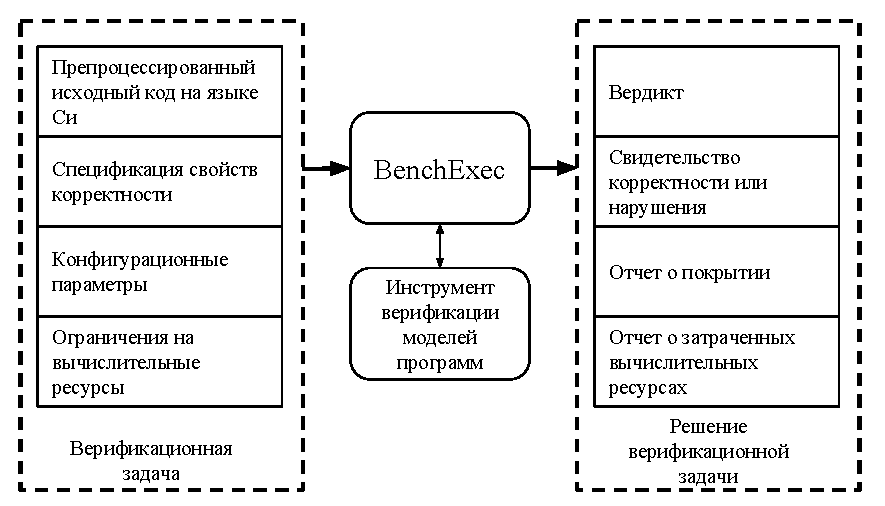
\includegraphics[scale=1]{BenchExec}
\caption{Схема решения верификационных задач.}
\label{figure:benchexec}
\end{figure}

Описание верификационной задачи представляет собой XML файл, который содержит пути к файлам с исходным кодом и спецификацией свойств корректности.
Верификационная задача может дополнительно содержать ограничения на вычислительные ресурсы и конфигурационные параметры для запуска конкретного инструмента верификации моделей программ, но формат не предусматривает единого способа задания конфигурационных параметров в едином виде для разных инструментов верификации.

Отчет о решении верификационной задачи содержит вердикт, пути к файлам свидетельств корректности или нарушения, отчет о покрытии и отчет о затраченных вычислительных ресурсах, включая время решения верификационной задачи, процессорное времени, максимальный объем используемой оперативной и дисковой памяти во время решения.

Вердикт --- это главный результат решения верификационной задачи, который может принимать значения \textbf{True}, \textbf{False} или \textbf{Unknown}.
Значение True означает, что выполнение свойств корректности доказано.
В этом случае инструмент выдает файл свидетельства корректности (англ. correctness witness).
Вердикт False соответствует обнаружению такого ошибочного пути выполнения программы (контрпримера), который опровергает тезис о выполнении свойства корректности.
Инструмент выдает ошибочный путь, содержащий предположения о значении переменных при выполнении инструкций программы, в виде файла свидетельства нарушения (англ. violation witness).
Если инструмент верификации моделей программ не смог доказать или опровергнуть выполнение свойств корректности при заданных ограничениях на вычислительные ресурсы, то вердикт принимает значение Unknown.

BenchExec использует механизм \textit{cgrpoups}~\cite{cgroups} ядра операционной системы Linux для ограничения и подсчета потребляемых процессорного времени и оперативной памяти, а для ограничения дисковой памяти и доступа к файловой системе используются возможности файловой системы \textit{Overlay}~cite{overlay}.
BenchExec останавливает выполнение инструмента при превышении им ограничения на доступные вычислительные ресурсы и в этом случае выдает вердикт Unknown.

Отчет о покрытии отражает ту часть кода, которая достижима из точки входа (функции \textit{main}).
При верификации небольших замкнутых программ, данный отчет обычно не несет большой практической пользы, так как инструменты верификации моделей программ анализируют все пути выполнения, возможные в программе.
Поэтому только некоторые инструменты верификации моделей программ в составе результатов решения верификационной задачи включают файл отчета о покрытии исходного кода программы~\cite{verificationcov}.
Но при верификации модулей программных систем, которые могут не являться замкнутыми программами и иметь несколько точек входа, данный отчет позволяет определить недостатки верификационной задачи, в частности неполноту модели окружения, которая рассмотрена в следующем разделе.

\subsection{Поддержка языка Си}
%Инструменты верификации моделей программ строят модель на основе исходного кода.
Для верификации программ на различных языках программирования инструменты используют специальное внутреннее представление.
Например, инструмент верификации моделей программ Corral опирается на инфраструктуру SMACK для трансляции программ во внутреннем представлении LLVM в программу на языке Boogie~\cite{tacas2015-hcelqr}.
А для работы с программами на языке программирования Си в инструменте CPAchecker~\cite{Beyer:2011:CTC} используется парсер Eclipse CDT.

Инструменты верификации моделей программ реализуют различные методы, но имеют схожие ограничения при верификации программ на языке Си:
\begin{itemize}
    \item фрагменты программы на языке ассемблера не поддерживаются большинством инструментов верификации моделей программ. Если программа содержит такие фрагменты, то либо инструменты игнорируют данный код (анализируют программу в предположении, что данный фрагмент на языке ассемблера не влияет на корректность программы), либо аварийно завершают свою работу.
    \item Инструменты, которые реализуют метод ограничиваемой проверки моделей~\cite{Biere03boundedmodel}, проверяют пути выполнения программы с фиксированным числом итераций и определенной глубиной рекурсии. Другие методы верификации моделей могут не иметь такого ограничения, например, метод k-индукции позволяет анализировать циклы любой длины~\cite{kinduction}.
    \item Инструменты верификации моделей программ имеют разные ограничения при верификации арифметики с указателями, битовыми операциями, операциями с плавающей точкой, строками, массивами, функциональными указателями, списками и т.д. Один инструмент, как правило, может иметь несколько реализаций способов построения модели программы и видов анализа для верификации программы с необходимым уровнем точности. 
    \item Инструменты верификации поддерживают небольшой набор моделей функций стандартной библиотеки языка Си и каждый инструмент имеет собственный список таких моделируемых функций.
    \item Проверку некоторых требований инструменты верификации моделей программ могут выполнять только для последовательных программ.
    Направление верификации параллельных программ развивается и широко представлены инструменты для проверки программ, использующих интерфейс управления потоками согласно стандарту POSIX.
\end{itemize}

\subsection{формализация требований при помощи свойств корректности}
Спецификация свойств корректности содержит формулы темпоральной логики.
Проверка каждого свойства корректности задается при помощи следующего выражения:

\[CHECK( init(main()), LTL(\phi) )\]

При верификации моделей программ анализируются все возможные пути выполнения, которые начинаются из функции \textit{точки входа}.
Имя такой функции указывается в качестве первого аргумента $CHECK$.
В данном примере точкой входа является функция \textit{main}.
Формула $\phi$ соответствует проверяемому свойству корректности и может принимать следующий вид:
\begin{itemize}
\item $\mathbf{G}~!call(\_\_VERIFIER\_error())$ --- свойство недостижимости ошибочного оператора (в данном примере вызова функции \textit{\_\_VERIFIER\_error});
\item $\mathbf{G}~!overflow$ --- свойство непереполнения целочисленного знакового типа;
\item $\mathbf{G}~valid-free$, $\mathbf{G}~valid-deref$, $\mathbf{G}~valid-memtrack$ --- свойство безопасного доступа к памяти, выраженное в виде совокупности трех формул.
\item $\mathbf{F}~end$ --- свойство завершимости.
\end{itemize}

На практике задачу проверки какого-либо требования к программе сводят к проверке одного или нескольких поддерживаемых свойств корректности.
Для этого разрабатывается модель требования на языке программирования Си для добавления к исходному коду верификационной задачи, в том числе и при помощи инструментации оригинального исходного кода верифицируемой программы.
При проверке таких требований, как, например, завершимость программы или корректность работы с памятью такая модель может быть тривиальной или не требоваться вовсе, если инструмент верификации поддерживает проверку соответствующего свойства корректности.
Для функциональных требований или программных контрактов, как правило, нужно разработать существенно более сложную модель требования для сведения задачи к доказательству выполнения свойства недостижимости ошибочного оператора.

Отдельные инструменты верификации моделей программ поддерживают другие способы формализации требований, основанные на спецификации требования при помощи некоторого языка предметной области или формализма.
Например, в инструменте верификации CPAchecker можно задать модель некоторых требований в виде автомата~\cite{Apel:2016}, но такой подход не позволяет применять другие инструменты верификации.

Инструменты верификации моделей программ выполняют анализ верификационной задачи до первого найденного нарушения свойства корректности.
Данная особенность обусловлена тем, что инструменты предназначены для доказательства корректности всей программы в составе верификационной задачи, а не отдельных функций или блоков кода.
Эксперименты по повторному использованию результатов верификации нескольких свойств корректности и требований ведутся разными командами исследователей~\cite{CPAreuse, CMBCreuse, Apel:2016}. 
На практике это затрудняет разработку моделей требований и может привести к ухудшению результатов, если какая-либо модель требования недостаточно точна и приводит к большому числу ложных срабатываний или требует слишком много вычислительных ресурсов для проверки.

В данной работе рассматривается проверка только таких требований, для любых нарушений которых может быть найден ошибочный путь (контрпример) конечной длины.
Из рассмотренных свойств корректности к таким не относится только свойство завершимости.

\subsection{Моделирование окружения}
Инструменты верификации моделей программ предназначены для верификации замкнутых программ на языке программирования Си.
Такие программы имеют одну точку входа, например, функцию \textit{main} и опираются только на стандартную библиотеку языка Си.

На практике программы и в особенности их отдельные модули взаимодействуют с окружением, в которое входят другие модули программы и операционная система.
Для верификации такого модуля программы требуется специфицировать предположения о взаимодействии модуля с окружением.
Для этого следует, как правило, разработать модель окружения на языке Си.
Такая модель содержит недостающие определения функций и реализует искусственную точку входа, если верифицируемый модуль программы не содержит функции \textit{main} и определяет несколько функций, вызываемых в окружении.
%Вызов точек входа в модели должен выполняться согласно устройству окружения программы.

Сообщество разработчиков SV"~COMP не предоставляет специальных средств для автоматизации или сокращения трудоемкости разработки моделей окружения.
Наиболее распространенный подход при моделировании --- это разработка модели окружения в виде отдельных фрагментов на языке программирования Си и инструментация исходного кода автоматически или вручную для добавления данных фрагментов в исходный код модуля.

Неточность и неполнота модели окружения может приводить и к пропуску ошибок, и к ложным предупреждениям об ошибках.
Исследователи подтверждают, что моделирование окружения на практике необходимо при верификации отдельных модулей программных систем и может требовать значительных усилий~\cite{subsystems:Trudy, ZakharovEnv2015, ModelingLargeSystems, neville2016a, FlashDriver, ConcurBugsRakamaric, Ivancic:2015:SSS}.
В то же время для поиска ошибок, а не для формальной верификации, сложность модели окружения может быть значительно снижена по сравнению с устройством реального окружения~\cite{ZakharovEnv2015}.

Некоторые неопределенные функции из стандартной библиотеки языка программирования Си поддерживаются инструментами верификации моделей программ и не требуют явного моделирования.
Для остальных неопределенных функций без разработанной вручную модели инструменты верификации предполагают возвращение неопределенного значения в соответствии с сигнатурой функции и отсутствие побочных эффектов, то есть выполнение функции без изменения значений аргументов, глобальных переменных и памяти во время выполнения.

При моделировании окружения программ на языке программирования Си используются специальные функции, поддерживаемые инструментами верификации, разрабатываемыми в рамках сообщества SV"~COMP.
Например, функция \textit{\_\_VERIFIER\_nondet\_int} возвращает неопределенное целое число, что упрощает моделирование неопределенного поведения окружения.
Полезной при моделировании окружения является функция \textit{\_\_VERIFIER\_assume}.
Единственным аргументом данной функции служит логическое выражение над переменными программы.
Пути, на которых выражение принимает ложное значение, не могут служить контрпримерами для выдачи предупреждений об ошибках.
Некоторые инструменты верификации моделей программ поддерживают более широкий набор функций для моделирования окружения.
Например, режим работы инструмента CPAchecker с анализом символических графов памяти (SMG) позволяет использовать функции \textit{external\_allocated\_data} для обозначения внешней <<корректной>> памяти, выделенной в модели окружения, и ошибки, связанные с некорректным доступом к такой памяти, игнорируются.

\subsection{Требования к вычислительным ресурсам}
При проверке программы с большим количеством циклов, ветвлений или потоков возникает проблема взрыва числа состояний в модели, построенной инструментом верификации для проверки требования на основе исходного кода данной программы.
О существовании метода оценки объема требуемых вычислительных ресурсов для успешного завершения верификации автору не известно.
Сколько потребуется вычислительных ресурсов зависит от многих факторов, например, от проверяемых свойств корректности, конфигурационных параметров инструмента, используемого SMT решателя, сложности исходного кода, производительности вычислительной системы.
Инструменты реализуют разные способы построения модели и алгоритмы для ее верификации.
Снижение точности модели или анализа не приводит к пропуску нарушений требований, но способно вызывать ложные сообщения об ошибках. 
Выбор наиболее точных подходов, как правило, всегда приводит к существенному увеличению времени работы инструментов верификации.

При сравнительном анализе инструментов верификации моделей программ в рамках SV"~COMP на решение каждой верификационной задачи отводится 15 минут процессорного времени и 15 GB оперативной памяти.
Данных ограничений бывает достаточно для верификации программ размером несколько десятков тысяч строк кода на языке программирования Си.

\subsection{Оценка результатов верификации}
Для проверки корректности вердикта сообществом SV"~COMP предложен подход валидации свидетельств корректности и нарушений при помощи специальных инструментов верификации моделей программ --- \textit{валидаторов}~\cite{Beyer:2015:WVS,Beyer:2016:CWE}.
Для выявления ложных сообщений об ошибках свидетельства нарушений могут быть валидированы и при помощи генерации тестов для проверки выполнимости ошибочного пути динамически~\cite{Beyer2018TestsFW, Beyer:2004:GTC}.

При верификации модуля программы верификационная задача содержит модель требования и модель окружения.
Упомянутые методы валидации позволяют определить неверный вердикт, причиной которого может быть только неточный анализ инструмента верификации моделей программ.
Если некорректный вердикт получен из-за неточной или неполной модели окружения или требования, то необходимо выполнение экспертизы свидетельств пользователем.

Свидетельства корректности и нарушения предназначены для валидаторов, которые в составе входных данных получают исходный код верификационной задачи.
Поэтому инструменты опускают важные фрагменты ошибочных путей при выдаче свидетельств нарушения, а для свидетельств корректности предоставляют только инварианты циклов программы.
Следовательно, даже с использованием средств визуализации, без вспомогательной информации анализ свидетельств вручную является трудным.

BenchExec предоставляет средство визуализации свидетельств нарушений, которое, однако, имеет ряд недостатков:
\begin{itemize}
    \item низкая масштабируемость и визуализация только простых ошибочных путей длиной несколько сотен строк кода;
    \item невозможность отличить код моделей окружения и требований от оригинального исходного кода верифицируемой программы;
    \item отсутствие связи между препроцессированным исходным кодом верификационной задачи и исходным кодом программы до препроцессирования;
    \item отсутствие подсказок и сообщений для пользователя о причине и вероятном месте ошибки в программе.
\end{itemize}

\section{Ограничения подходов к применению инструментов верификации моделей Си-программ}
% Применение инструментов на практике CBMC
Инструменты верификации моделей программ применяются для проверки требований различных программных систем на языке программирования Си:
\begin{itemize}
    \item При помощи CMBC была проверена реализация алгоритма сжатия\break Brotli\cite{brotli} и показана возможность обнаружения известной уязвимости~\cite{neville2016a}.
    \item Инструмент CMBC используется для генерации тестов в рамках системы BTC EMBEDDEDTESTER для тестирования встраиваемого программного обеспечения~\cite{CMBCreuse}. CBMC применялся для верификации операционной системы TinyOS и другого программного обеспечения для встраиваемых систем~\cite{Schlich2009, Bucur:2010:SVT}. Также инструменты СBMC и CPAchecker были интегрированы в среду для разработки встраиваемого программного обеспечения $mbeddr$~\cite{mbeddr}. 
    \item Ряд работ рассматривает верификацию драйверов~\cite{Post:2009:TAS,Witkowski:2007:MCC, ModelingLargeSystems, FlashDriver, ConcurBugsRakamaric} и файловых систем~\cite{Galloway:2008:MLV, Yang:2006:UMC}.
    \item При помощи CMC была выполнена проверка реализации сетевого протокола TCP в ядре операционной системы Linux~\cite{Musuvathi:2004:MCL}.
    \item Известны примеры верификации моделей программ на языке Си++. Например, ESBMC++ предлагается использовать для проверки приложений на основе фреймворка Qt~\cite{QTverification}.
\end{itemize}

Перечисленные работы нацелены на поиск ошибок, а не на доказательство корректности модулей Си-программ.
Полученные результаты подтверждают возможность обнаружения ошибок в крупных программных системах на языке программирования Си.
В то же время, работы выполнялись разработчиками инструментов верификации или исследователями с хорошей математической подготовкой.
В процессе верификации требуется модифицировать исходный код, моделировать окружение и требования, изучать ложные срабатывания, устранять их причины.
В большинстве работ весь процесс верификации детально не описан и трудозатраты не представлены.
В некоторых случаях отдельные шаги процесса верификации были автоматизированы, но авторы не предложили каких-либо средств, применимых при верификации другого программного обеспечения.

Основную сложность при подготовке программ к верификации составляют шаги моделирования окружения и формализации требований.
Модели окружения в перечисленных работах разрабатываются на языке Си.
Например, некоторые авторы признают, что только для разработки модели окружения отдельного драйвера операционной системы вручную может требоваться около одного человеко-месяца~\cite{ConcurBugsRakamaric}.
Еще одним ограничением подхода разработки моделей вручную на языке Си является возможность проверять только определенный тип требований.
Например, если модель окружения разработана для применения инструмента верификации моделей программ для проверки требований, сведенных к доказательству недостижимости ошибочного оператора в последовательной программе, то для поиска гонок по данным придется разрабатывать новую параллельную модель окружения.
Схожие ограничения имеет подход, предложенный для поиска ошибок в драйверах при помощи символьного выполнения и реализованный в инструменте SymDrive~\cite{Renzelmann:2012:STD}.
Для применения инструмента также требуется разработать вручную модель окружения на языке программирования Си, которая применима только при поиске ошибок определенного вида.

Для описания моделей различных систем применяется множество языков и формализмов~\cite{Seshia2018}.
Но для применения инструментов верификации моделей Си-программ верификационная задача должна включать исходный код именно на языке программирования Си.
По этой причине на практике не используются подходы к моделированию окружения, которые предполагают описание модели окружения на языке, значительно отличающемся от языка Си по синтаксису или семантике.

Еще одним направлением применения метода проверки моделей для проверки программного обеспечения является композиционная верификация программ на языках Си\IntroCite{LTSA} и Java\IntroCite{Giannakopoulou:2004:AVS, Parizek:2007:SGE, Zhai:2016:AMG,parizek2007partial,Tkachuk:2003:AEG} на основе спецификаций предположений об окружении.
Отличительной особенностью данных работ является цель доказать корректность целевого модуля или программы формально.
Трудоемкость композиционной верификации велика и доказательства корректности могут быть получены только для небольших программ или модулей.
Для описания моделей окружения используется либо непосредственно язык программирования, на котором разработана программа, либо некоторые языки предметной области, которые позволяют описать ограничения на последовательность вызова точек входа модуля в виде спецификации.
Предложенные методы синтеза моделей окружения на основе таких спецификаций позволяют снизить трудоемкость подготовки моделей окружения для классов на языке Java, но не учитывают особенностей устройства интерфейса программ на языке Си.

Для автоматизированного применения инструментов верификации моделей Си-программ для проверки требований к модулям крупных программных систем требуется автоматизировать синтез верификационных задач.
В этом случае возникает задача декомпозиции программы на модули, состоящие из наборов файлов с исходным кодом на языке программирования Си.
Схожие формулировки задачи декомпозиции программы встречаются и в других предметных областях, например, в работах, посвященных рефакторингу.
Отличительной особенностью задачи декомпозиции в области верификации моделей программ является трудность формализации критериев, которым должны удовлетворять полученные после декомпозиции модули программы.
Автору неизвестно о работах, которые предложили бы метод проверки с достаточным уровнем точности возможности успешного решения верификационной задачи, полученной на основе некоторого модуля программы.
Как было ранее упомянуто при рассмотрении вопроса масштабируемости инструментов верификации, процесс верификации зависит от множества факторов.
Схожая трудность возникает при попытке оценить трудоемкость разработки моделей окружения для заданного модуля.
Число точек входа и неопределенных функций в модуле лишь косвенно влияет на трудоемкость разработки таких моделей.
Поэтому задача декомпозиции для каждой верифицируемой программной системы решается с учетом устройства ее модулей и о попытках обобщить полученные результаты для декомпозиции программ, имеющих разный вид и устройство, автору не известно.

Для автоматизированного применения инструментов верификации моделей программ были реализованы системы верификации.
Системы верификации LDV Tools~\cite{Zakharov2015} и SDV~\cite{Ball2004} нацелены на проверку требований корректного использования интерфейса ядра операционной системы (ОС) в драйверах Linux и Windows соответственно.
Система верификации DC2~\cite{Ivancic:2015:SSS} позволяет проверять требование корректности работы с памятью к программному обеспечению встраиваемых систем.

% Система статической верификации драйеров Windows
Система верификации SDV была включена в состав набора средств для разработки драйверов Microsoft Windows Driver Development Kit в 2006 году.
SDV может быть использована в качестве плагина среды разработки Visual Studio.
Исходный код системы верификации является закрытым.

% Подготовка драйвера и Модель окружения
Система поддерживает верификацию драйверов устройств ОС Windows определенных типов.
Для таких типов были разработаны модели окружения на языке программирования Си вручную.
Модели позволяют проверять исходный код драйверов обработки IRP запросов и драйверов минипорта для сетевых устройств отдельно от исходного кода ОС Windows.
Обработчики проверяемого драйвера, которые являются его точками входа, должны быть аннотированы пользователем вручную.

В состав системы верификации входит несколько сотен спецификаций требований.
Для их задания используется аспектно-ориентированное расширение языка программирования Си SLIC (англ. Specification Language for Interface Checking)~\cite{SLIC}.
Язык схож с языком Си по синтаксису, поэтому в разработке спецификаций корректности использования интерфейса ядра драйвером участвуют не только эксперты в области верификации.

% Инструмент верификации
Первоначально в системе применялся инструмент верификации моделей программ SLAM~\cite{Ball:2011:DSM}.
Затем стало возможным использование инструментов SLAM2~\cite{SLAM2}, Yogi~\cite{Yogi} и Q, основанном на CORRAL~\cite{Lal:2014:PSD}. 
Перечисленные инструменты не поддерживают предложенные в SV"~COMP форматы верификационных задач.

% Вывод
Система верификации SDV имеет высокую практическую значимость:
\begin{itemize}
\item Система верификации используется не только специалистами в области верификации, но и разработчиками драйверов ОС Windows.
\item Результаты верификации имеют крайне низкий процент ложных сообщений об ошибках. 
В работе о SLAM2 сообщается, что этот показатель составляет 4\%~\cite{SLAM2}.
\item По состоянию на 2010 год при помощи системы верификации было выявлено 270 ошибок, что существенно повысило надежность драйверов операционной системы Windows, согласно утверждениям разработчиков системы верификации.
\end{itemize}

% Система статической верификации драйверов Linux LDV Tools
В рамках проекта LDV (англ. Linux Drivers Verification) по верификации драйверов ядра ОС Linux, который начался в 2012 году, была разработана система верификации LDV Tools~\cite{configurable:Trudy, Zakharov2015, Beyer:2012:LDV}.

Система верификации выполняет синтез моделей окружения и моделей требований.
Для синтеза моделей окружения используется подход вызова обработчиков драйверов на основе шаблонов.
При помощи шаблонов могут быть заданы ограничения на порядок вызова обработчиков, но описать ограничения на параметры при вызове реализованный подход не позволяет.
Процесс подготовки моделей окружения не предполагает возможности проверки разных свойств корректности, отличных от свойства недостижимости ошибочного оператора.

Система статической верификации позволяет проверять несколько десятков специальных требований корректности использования интерфейса ядра в драйверах, например, корректность синхронизации процессов, инициализации, захвата и освобождения различных ресурсов, передачи параметров функциям ядра в зависимости от контекста выполнения.
Каждое требование формализовано в виде контрактной спецификации на аспектном расширении языка Си.
Для синтеза верификационных задач исходный код драйвера инструментируется при помощи инструмента CIF для добавления моделей окружения и требований к исходному коду драйверов~\cite{Novikov2013}.

Система верификации позволяет использовать инструменты верификации моделей программ CBMC, CPAchecker и Blast, разрабатываемые и поддерживаемые сообществом SV"~COMP.
Но инструмент BenchExec в системе не используется, поэтому для применения инструментов разработаны адаптеры для конвертирования входных и выходных данных в необходимые форматы.

Одним из главных недостатков системы является низкая масштабируемость.
Система верификации не позволяет синтезировать верификационные задачи параллельно, что значительно увеличивает время получения результатов.
Например, для верификации всех модулей ядра Linux, которых в исходном коде ядра порядка четырех тысяч, на соответствие одному требованию требуется более суток.
Архитектура системы верификации имеет ряд важных ограничений, например, систему не может использовать несколько пользователей одновременно, что при высоких требованиях к вычислительным ресурсам затрудняет ее использование в рамках распределенных вычислительных систем.

Система верификации позволила найти более 200 ошибок в драйверах ОС Linux, которые были подтверждены их разработчиками.
В то же время число ложных предупреждений об ошибках в результатах верификации достаточно велико.
Согласно результатам, представленным в работах~\cite{configurable:Trudy, Zakharov2015}, 60\% ложных сообщений об ошибках вызваны именно неточностью моделей окружения, для исправления которых в системе не предусмотрено необходимых средств.

% Система верификации DC2
Система верификации DC2 нацелена на проверку требований корректности работы с памятью к программному обеспечению встраиваемых систем ~\cite{Ivancic:2015:SSS}.
Система является закрытым проектом, разрабатываемым компанией NEC.

% Модель окружения
Система верификации реализует метод уточнения модели окружения по контр-примеру CEGER (англ. Counter-Example Guided Environment Refinement).
Перед верификацией система выполняет легковесный межпроцедурный статический анализ исходного кода программы \textsc{SpecTackle}.
Анализ нацелен на генерацию моделей окружения с условиями (англ. constraints) для разных точек программы, например, предусловий или постусловий вызова функций.
Анализ выделяет условия, связанные с разыменованием указателей, выделением памяти, обращениями к массивам.
Модель окружения генерируются в виде аннотаций к исходному коду.
\textsc{SpecTackle} опирается на различные эвристики и может генерировать некорректные модели окружения.
Предполагается, что пользователь может исправить модели окружения вручную, выполняя процесс верификации итеративно.
Данный подход автоматизирует подготовку модели окружения для программ размера несколько сотен тысяч строк кода на языке Си.
Предложенный метод нацелен на замену функций на их упрощенные заглушки, но не позволяет генерировать вызовы точек входа.
Данным недостатком обладают и методы верификации программ с ограничением области видимости (англ. scope-bounded verification) и межпроцедурного статического анализа.

В качестве единственного инструмента верификации используется VARVEL, разрабатываемый корпорацией NEC.
Инструмент в системе верификации используется для проверки свойства корректности работы с памятью и позволяет обнаруживать такие дефекты, как, например, выход за границу массива, повторное освобождение памяти, утечки памяти.

% Анализ результатов
Сообщается об успешном пилотном применении системы верификации разработчиками компании для проверки проектов размера более сотни тысяч строк кода.
В рамках применения системы верификации удалось обнаружить и исправить более десятка ошибок. 
Так как проект является закрытым, то оценить в полной мере применимость предложенных методов для верификации различных программ на языке программирования Си не удается.

\begin{table}
\centering
\begin{tabular}{ | l | c | c | c | }
\hline
Критерий сравнения & SDV & LDV & DC2 \\
\hline
\begin{tabular}{@{}l@{}} Поддержка адаптивной декомпозиции программ\end{tabular} & \ding{55} & \ding{55} & \ding{55} \\
\hline
\begin{tabular}{@{}l@{}} Наличие средств для разработки или \\ исправления моделей окружения  \end{tabular} & \ding{51} & \ding{55} & \ding{55} \\
\hline
\begin{tabular}{@{}l@{}} Синтез моделей окружения\end{tabular} & \ding{55} & \ding{51} & \ding{51} \\
\hline
\begin{tabular}{@{}l@{}} Наличие средств для разработки или \\ исправления моделей требований \end{tabular} & \ding{51} & \ding{51} & \ding{55} \\
\hline
\begin{tabular}{@{}l@{}} Синтез моделей требований \end{tabular} & \ding{51} & \ding{51} & \ding{51} \\
\hline
\begin{tabular}{@{}l@{}} Поддержка проверки разных свойств корректности\end{tabular} & \ding{55} & \ding{55} & \ding{55} \\
\hline
\end{tabular}
\caption{Сравнение систем верификации моделей программ.}
\label{table:systems}
\end{table}

В таблице~\ref{table:systems} представлено сравнение систем верификации моделей программ.
Рассмотренные системы верификации не предлагают средств автоматизации декомпозиции программ разных видов.
Средства для разработки моделей окружения, в которых можно задать и вызов точек входа, и модели отсутствующих функций, реализованы только в SDV, но разработка моделей окружения предусмотрена только на языке Си.
Системы верификации нацелены на проверку конкретных видов требований к определенным программным системам и не предполагают возможности адаптировать процесс синтеза верификационных задач для верификации других программных систем.
Системы верификации LDV и SDV позволяют проверять выполнение только свойства недостижимости ошибочного оператора, а DC2 только свойства корректности работы с памятью.
LDV, и SDV реализуют подходы для сведения проверки различных требований к проверке свойства недостижимости ошибочного оператора.

Согласно рассмотренным работам, при применении инструментов верификации моделей Си-программ для проверки требований к крупным программным системам основными ограничениями остаются отсутствие методов автоматизации декомпозиции программ разных видов и высокая трудоемкость моделирования окружения.
Существующие системы верификации, предназначенные для автоматизации применения инструментов верификации, не предусматривают адаптации процесса синтеза верификационных задач для различных программных систем и для проверки требований к ним, формализованных на основе различных свойств корректности.

\section{Методы распараллеливания верификации моделей программ}

Инструменты верификации моделей программ реализуют, как правило, последовательные алгоритмы верификации моделей.
Они не используют преимуществ многоядерных и графических процессоров или распределенных вычислительных систем.
Применение инструментов верификации для проверки требований к крупным программным системам на языке Си может требовать решения большого числа верификационных задач, что подтверждается опытом практического применения систем верификации LDV и SDV.
Поэтому следует рассмотреть методы сокращения времени решения совокупности верификационных задач и каждой задачи в отдельности.
За последние годы появилось много примеров применения высокопроизводительных вычислений (англ. high-perfromance computing) в области верификации моделей~\cite{survey:new}.
Чтобы определить на какие вычислительные системы впоследствии могут быть рассчитаны инструменты верификации моделей программ, требуется рассмотреть исследования в данной области. 

% Кластеры
\subsection{Распределенные вычислительные системы}
Распределенные вычислительные системы (вычислительные кластеры) широко используются для повышения производительности различных приложений.
Параллельные версии алгоритмов для верификации моделей с применением вычислительных кластеров были предложены до появления инструментов верификации моделей программ.
Например, параллельная реализация инструмента верификации моделей Mur$\varphi$ была представлена уже в 1997 году~\cite{Stern97parallelizingthe}.
Алгоритм, представленный в работе, предполагает распределение частей пространства состояний проверяемой модели для обработки между узлам вычислительного кластера при помощи хэш-функции.
Другим примером применения распределенных вычислительных систем является работа, опубликованная в 1999 году разработчиками инструмента SPIN~\cite{Lerda1999}.
Инструмент DiVinE реализует результаты современного исследования в данной области~\cite{VW86b}.
Авторы представили версии алгоритмов как для распределенных вычислительных систем, так и для многоядерных процессоров с общей памятью ~\cite{Barnat:2010:SSM,HiBi.2009,Barnat2009,Barnat5161000}.
Наилучшее ускорение составило 8 раз относительно последовательной версии инструмента при использовании 10 узлов распределенной вычислительной системы.

Многие инструменты верификации моделей программ реализуют алгоритм уточнения абстракции по контрпримеру~\cite{Clarke:2003:CAR}.
Параллельная версия данного алгоритма для верификации моделей реализована в инструменте ARMC~\cite{Lopes2011}.
Алгоритм, представленный в работе, подразумевает использование одного главного и нескольких рабочих узлов.
Главный узел выполняет интерполяцию, проверку выполнимости формулы пути и хранит граф пространства состояний модели программы.
Рабочие узлы выполняют обход подмножества пространства состояний, полученного от главного узла, и отправляют результат работы на главный узел после расчета новых состояний.
Авторы уделили внимание проблеме воспроизведения результатов.
Наибольшее ускорение составило 28 раз относительно последовательной версии алгоритма при использовании вычислительного кластера из 40 узлов.

Облачные сервисы представляют собой масштабируемую распределенную систему, число задействованных узлов в которой может изменяться в зависимости от сложности решаемой задачи.
Универсальными облачными являются сервисы IaaS (англ. infrastructure as a service) и PaaS (platform as a service).
Сервисы IaaS позволяют получить распределенную вычислительную систему, состоящую из виртуальных машин с заданными характеристиками в качестве вычислительных узлов.
Примером такого сервиса является Amazon Elastic Cloud EC2~\cite{ec2}.
Альтернативным решением являются PaaS облачные сервисы, которые предоставляют пользователю возможность запускать экземпляры целевого приложения, обрабатывающие независимые запросы, в специальной вычислительной среде.
Сервис динамически регулирует число активных экземпляров приложения в зависимости от числа ожидающих обработки запросов.
Примером такой системы является Google App Engine~\cite{gae}.

% А также верификацию в PAAS GAE
Инструмент верификации моделей программ CPAchecker был адаптирован для запуска в облачном сервисе Google App Engine~\cite{Beyer:2014:SVG}. 
Для этого потребовалось отказаться от запуска вспомогательных сторонних компонентов в рамках работы инструмента, а также использовать заданный интерфейс для доступа к ресурсам операционной системы, например, к дисковой памяти.
Основным недостатком использования данного облачного сервиса на практике является запрет на задание достаточно высоких ограничений на вычислительные ресурсы, из-за чего верифицировать модули программ размером десятки тысяч строк кода на языке Си не удается.

Существуют также и специальные облачные сервисы, нацеленные на решение конкретной задачи в заданной предметной области.
Проект VerifierCloud~\cite{VerifierCloud} представляет собой облачный сервис, который также управляет вычислительным кластером для запуска инструментов верификации моделей программ изолированно на разных вычислительных узлах.
Данный проект широко используется для выполнения сравнительного анализа инструментов верификации моделей программ сообществом SV"~COMP~\cite{SVCOMP2014,Beyer2016}.
Разработчики также предоставляют специальный облачный сервис для решения верификационных задач при помощи инструмента CPAchecker.

% Многоядерные системы 
\subsection{Многоядерные вычислительные системы}
Современные процессоры имеют несколько ядер c функцией одновременной многопоточности (англ. simultaneous multithreading — SMT).
Для того, чтобы полноценно использовать многоядерную архитектуру необходимо реализовать параллельные алгоритмы, эффективно использующие разделяемую память.

Разработчики инструментов верификации моделей представили ряд работ по применению параллельных алгоритмов для работы с разделяемой памятью. 
Алгоритмы реализованы в таких инструментах, как SPIN~\cite{Holzmann:2003:SMC,5661793,Holzmann:2012:PSM}, DiVinE~\cite{Brim2001,BARNAT2003,Brim2004,Brim:2006:OVD,Barnat:2010:SSM} и LTSmin~\cite{Laarman2011,Laarman:2010:BMR}.
В представленных работах авторы уделили внимание проблеме реализации структур данных для хранения пространства состояний и параллельного доступа к ним из разных потоков.
При использовании многопоточных процессоров нехватка памяти при верификации снова выходит на первый план.
Для преодоления данной проблемы в SPIN было реализовано сокращение частичных порядков~\cite{Bosnacki2006}, а разработчики LTSmin предложили алгоритм Collapse для сжатия данных~\cite{Laarman2011mem}.

В рассмотренных работах были достигнуты различные результаты.
Но в все инструменты смогли достигнуть ускорения порядка 5-10 раз при эффективности (отношение ускорения к числу потоков) 50\% при использовании до 10-30 потоков.

\subsubsection{Графические процессоры}
Успехи в разработке высокопроизводительных графических процессоров привели к широкому их распространению для организации вычислений в различных сферах.
А появление такой платформы как NVIDIA CUDA сделало применение графических процессоров менее трудоемким~\cite{cuda}.
Автору не известны применения графических процессоров для верификации моделей программ, но результаты экспериментов по верификации моделей при помощи данной аппаратуры уже опубликованы разными командами исследователей.

Современные графические процессоры обладают высокой производительностью, но имеют свои отличительные особенности.
Графические процессоры адаптированы под операции с данными в матрично-векторной форме.
Исходный код отличается от кода для центрального процессора.
Из-за более длительного такта системные вызовы и ожидания при выполнении существенно снижают производительность.
Кроме того, графические процессоры обладают своей иерархией памяти и объем соответствующей разделяемой памяти обычно значительно меньше, чем объем оперативной памяти.

Разработчики инструмента DiVinE представили ряд работ, посвященных применению графических процессоров при проверке моделей~\cite{Barnat2009CUDA,Barnat2010CUDA,Barnat2012CUDA}.
Авторы адаптировали алгоритм MAP к матрично-векторной форме, а также реализовали параллельное выполнение центральным процессором поиска допускающего цикла.
В работе сообщается об ускорении в среднем в пять раз относительно последовательной версии инструмента, использующей только центральный процессор.
В работе, посвященной вероятностной верификации моделей (англ. probabilistic model checking), предлагается использовать обратную польскую запись~\cite{Burks:1954:ALM} для описания изменения состояний в модели~\cite{Bosnacki2009}.
Реализация алгоритма с использованием NVIDIA CUDA в инструменте SPIN представлена в работе~\cite{Bartocci:2014:TGS}.
Авторы сообщают также об ускорении до 7 раз по сравнению с последовательной версией алгоритма для центрального процессора.
Еще одним примером вероятностной проверки моделей является реализация инструмента PRISM~\cite{Kwiatkowska2002,Bosnacki:2010:GEP}.
Ряд работ опубликовали разработчики инструмента GPUexplore, нацеленного на верификацию моделей с явными значениями (англ. explicit state model checking)~\cite{Wijs2014,Wijs2016GPUexplore2U,Wijs2014,Neele2016}.
Авторы заявляют об ускорении верификации вплоть до 100 раз.

Результаты представленных выше работ демонстрируют возможность существенно сократить время верификации моделей с использованием графических процессоров.
В то же время верификация моделей с большим числом состояний при помощи графических процессоров затруднительна из-за ограниченного объема доступной памяти, и это ставит под сомнение эффективность данного направления для верификации моделей программ.
Чтобы достичь высокой производительности необходимо оптимизировать представление данных, что требует от разработчика хорошего понимания устройства иерархии памяти в графических процессорах, которая также развивается с появлением новых версий аппаратуры.

\subsection{Выводы}
Для сокращения времени решения верификационных задач при автоматизированном применении инструментов верификации моделей программ для проверки требований к крупным программным системам на языке программирования Си в данной работе предпочтение отдается методам распределенного параллельного решения верификационных задач с использованием вычислительных кластеров, IaaS платформ и специальных облачных сервисов.
Данный подход позволит применять как доступные сегодня инструменты верификации моделей программ, которые реализуют последовательные алгоритмы, так и инструменты, реализующие алгоритмы для многоядерных процессоров, эффективность которых показана в упомянутых работах по верификации моделей.

% Промежуточный вывод касательно верификационных задач SV"~COMP
\section{Требования к системе верификации моделей крупных программных систем на языке Си}
Данная работа посвящена развитию систем верификации моделей Си-программ для преодоления существующих ограничений, возникающих при их применении к крупным программным системам.
Для преодоления данных ограничений необходимо в первую очередь сократить трудоемкость подготовки верификационных задач и время их решения.
Для этого предлагается разработать новые методы автоматизированных декомпозиции Си-программ и синтеза моделей окружения, удовлетворяющие следующим требованиям:
\begin{itemize}
    \item Декомпозицию и синтез моделей окружения следует  автоматизировать таким образом, чтобы пользователь имел возможность выполнять адаптацию данных процессов, выполняемых при генерации верификационных задач, для разных программ и при проверке различных видов требований, предъявляемых к этим программам.
    Адаптацию предлагается выполнять при помощи конфигурирования и разработки спецификаций.
    \item Синтез моделей окружения следует выполнять на основе подготовленных вручную спецификаций предположений об окружении.
    Формат спецификаций должен позволять описывать и модели вызова точек входа модулей программ, и модели неопределенных функций.
    \item Для применения различных инструментов верификации моделей Си-программ следует использовать формат верификационных задач, разработанный сообществом SV"~COMP.
\end{itemize}

Предложенные методы предлагается реализовать в новой системе верификации, которая должна отвечать современным требованиям к системам такого класса.
В частности система должна обеспечивать следующие возможности:
\begin{itemize}
    \item Система верификации должна автоматизировать весь процесс верификации Си-программ, который включает этапы генерации верификационных задач, решения верификационных задач при помощи инструментов верификации и анализ результатов.
    \item Генерация и решение верификационных задач должны выполняться параллельно с использованием многоядерных процессоров для сокращения времени решения верификационных задач.
    \item Необходимо предусмотреть возможность применения распределенных вычислительных систем для параллельного решения верификационных задач.
    \item Требуется обеспечить воспроизводимость результатов верификации. 
    \item Система верификации должна предусматривать возможность одновременного использования несколькими пользователями. 
\end{itemize}
